%%%%%%%%%%%%%%%%%%%%%%%%%%%%%%%%%%%%%%%%%%%%%%%%%%%%%%%%%%%%%%%%%%%%%%%%%%%%%%%%%%%%%%%%%%%%%%%%%%%%%%%%%%%%%%%%%%%%%%%%%%%%%%%%%%%%%%%%%%%%%%%%%%%%%%%%%%%%%%%%%%%%%%%%%%%%%%

\UC{Checkout}

\begin{figure}[H]
    \centering
    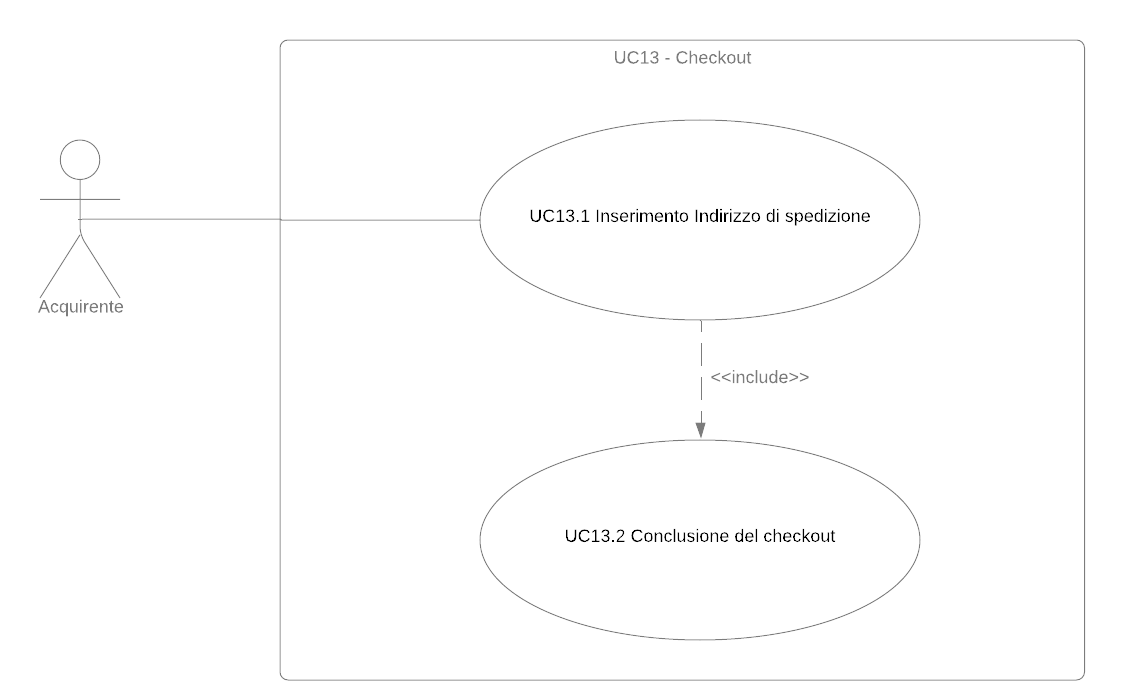
\includegraphics[scale=0.4]{Immagini/DiagrammiUC/UC13Checkout.png}
    \caption{Diagramma di \actualUC: Checkout} 
    \label{fig:Checkout}
\end{figure}

L'utente si trova nella schermata del carrello e vuole procedere al checkout per acquistare i prodotti scelti.
\begin{itemize}
    \item \textbf{Attori primari:} acquirente;
    \item \textbf{Attori secondari:} stripe;
    \item \textbf{Precondizione:} l'attore si trova nella schermata del carrello;
    \item \textbf{Postcondizione:} l'attore ha terminato il checkout e visualizza il riepilogo ordine.
    \item \textbf{Scenario principale:} l'attore si trova nella schermata del carrello e seleziona la funzionalità per procedere con il checkout. In seguito farà i seguenti passi:
    \begin{itemize}
    	\item sceglie l'indirizzo di spedizione, ovvero dove verrà recapitato l'acquisto;
    	\item sceglie la carta con la quale svolgere il pagamento.
        \item (\actualUC.1) - invia il pagamento.
    \end{itemize}
    \item \textbf{Scenario alternativo}: l'attore vuole svolgere l'operazione di checkout ma non è ancora autenticato. Per questo motivo verrà reindirizzato alla schermata di login per potersi autenticare come acquirente, per poi procedere in seguito al checkout. Se l'utente accede come venditore, il carrello con i prodotti salvati viene svuotato e andrà perso.
\end{itemize}

\resetSubUC

\subUC{Invio del pagamento}
L'acquirente procede al pagamento attraverso il servizio fornito da Stripe e poi gli viene mostrata una pagina con il resoconto dell'ordine.
\begin{itemize}
    \item \textbf{Attori primari:} acquirente e Stripe;
    \item \textbf{Precondizione:} l'acquirente non ha ancora pagato e il carrello non è vuoto;
    \item \textbf{Postcondizione:} l'acquirente ha effettuato il pagamento, il suo carrello è vuoto e si trova sulla pagina di riepilogo dell'ordine;
    \item \textbf{Scenario principale:}
        \begin{itemize}
            \item l'acquirente viene indirizzato alla pagina di checkout di Stripe, dove pagherà il costo del carrello più le spese di spedizione e le tasse;
            \item Stripe si occupa del pagamento;
            \item Quando è avvenuto il pagamento viene svuotato il carrello e gli articoli che lo componevano vengono sottratti nella quantità acquistata da quelli disponibili;
            \item Viene visualizzato il riepilogo ordine.
        \end{itemize}
    \item \textbf{Scenario alternativo:} Se il pagamento fallisce l'utente viene riportato alla pagina del carrello, senza che questo venga svuotato.
\end{itemize}

%%%%%%%%%%%%%%%%%%%%%%%%%%%%%%%%%%%%%%%%%%%%%%%%%%%%%%%%%%%%%%%%%%%%%%%%%%%%%%%%%%%%%%%%%%%%%%%%%%%%%%%%%%%%%%%%%%%%%%%%%%%%%%%%%%%%%%%%%%%%%%%%%%%%%%%%%%%%%%%%%%%%%%%%%%%%%%

\UC{Inserimento carta per pagamento}
L'acquirente è nella fase del checkout e vuole inserire una nuova carta da utilizzare per il pagamento.
\begin{itemize}
    \item \textbf{Attori primari:} acquirente;
    \item \textbf{Precondizione:} l'acquirente è nella fase del checkout e vuole inserire una nuova carta;
    \item \textbf{Postcondizione:} l'acquirente ha aggiunto la nuova carta da utilizzare per il pagamento;
    \item \textbf{Scenario principale:} l'acquirente è nella fase del checkout e vuole inserire una nuova carta. Per poterlo fare dovrà eseguire le seguenti azioni:
    \begin{itemize}
        \item (\actualUC.1) - inserimento dei dati della carta;
        \item conferma l'aggiunta della carta.
    \end{itemize}
\end{itemize}

\resetSubUC

\subUC{Inserimento dei dati della carta}
L'acquirente compila il modulo per aggiungere una nuova carta.
\begin{itemize}
	\item \textbf{Attori primari:} acquirente;
	\item \textbf{Precondizione:} l'acquirente si trova nella schermata di aggiunta di una nuova carta;
	\item \textbf{Postcondizione:} l'acquirente ha compilato correttamente tutti i dati della carta e può continuare con l'aggiunta;
	\item \textbf{Scenario principale:} l'acquirente compila i campi nel seguente modo:
	\begin{itemize}
		\item (\actualSubUC.1) - inserimento dell'intestatario della carta;
		\item (\actualSubUC.2) - inserimento del numero della carta;
		\item (\actualSubUC.3) - inserimento del CVV della carta;
		\item (\actualSubUC.4) - inserimento della data di scadenza della carta.
	\end{itemize}
\end{itemize}

\resetSubSubUC

\subSubUC{Inserimento dell'intestatario della carta}
L'acquirente inserisce l'intestatario della nuova carta da aggiungere.
\begin{itemize}
    \item \textbf{Attori primari:} acquirente;
    \item \textbf{Precondizione:} l'acquirente si trova nella schermata di aggiunta di una nuova carta;
    \item \textbf{Postcondizione:} l'acquirente ha inserito l'intestatario della carta da aggiungere;
    \item \textbf{Scenario principale:} l'acquirente inserisce correttamente l'intestatario della carta da aggiungere.
    \item \textbf{Estensioni:}
    \begin{enumerate}[label=\lett]
        \item l'utente non inserisce alcun intestatario della carta. In questo caso:
        \begin{itemize}
            \item (UC) - viene mostrato il messaggio d'errore campo dati obbligatorio non inserito;
            \item verrà impedita l'aggiunta della carta.
        \end{itemize}
    \end{enumerate}
\end{itemize}

\subSubUC{Inserimento del numero della carta}
L'acquirente inserisce il numero della nuova carta da aggiungere.
\begin{itemize}
    \item \textbf{Attori primari:} acquirente;
    \item \textbf{Precondizione:} l'acquirente si trova nella schermata di aggiunta di una nuova carta;
    \item \textbf{Postcondizione:} l'acquirente ha inserito il numero della carta da aggiungere;
    \item \textbf{Scenario principale:} l'acquirente inserisce correttamente il numero della carta da aggiungere;
    \item \textbf{Estensioni:}
    \begin{enumerate}[label=\lett]
        \item l'utente non inserisce alcun numero della carta. In questo caso:
        \begin{itemize}
            \item (UC) - viene mostrato il messaggio d'errore campo dati obbligatorio non inserito;
            \item verrà impedita l'aggiunta della carta.
        \end{itemize}
        \item l'utente non inserisce esattamente 16 numeri compresi tra 0 e 9 come numero della carta. In questo caso:
        \begin{itemize}
            \item (UC) - viene mostrato il messaggio d'errore numero della carta non valido;
            \item verrà impedita l'aggiunta della carta.
        \end{itemize}
    \end{enumerate}
\end{itemize}

\subSubUC{Inserimento del CVV della carta}
L'acquirente inserisce il CVV della nuova carta da aggiungere.
\begin{itemize}
    \item \textbf{Attori primari:} acquirente;
    \item \textbf{Precondizione:} l'acquirente si trova nella schermata di aggiunta di una nuova carta;
    \item \textbf{Postcondizione:} l'acquirente ha inserito il CVV della carta da aggiungere;
    \item \textbf{Scenario principale:} l'acquirente inserisce correttamente il CVV della carta da aggiungere.
    \item \textbf{Estensioni:}
    \begin{enumerate}[label=\lett]
        \item l'utente non inserisce alcun CVV della carta. In questo caso:
        \begin{itemize}
            \item (UC) - viene mostrato il messaggio d'errore campo dati obbligatorio non inserito;
            \item verrà impedita l'aggiunta della carta.
        \end{itemize}
        \item l'utente non inserisce esattamente 3 numeri compresi tra 0 e 9 come CVV della carta. In questo caso:
        \begin{itemize}
            \item (UC) - viene mostrato il messaggio d'errore CVV della carta non valido;
            \item verrà impedita l'aggiunta della carta.
        \end{itemize}
    \end{enumerate}
\end{itemize}

\subSubUC{Inserimento della data di scadenza della carta}
L'acquirente inserisce la data di scadenza della nuova carta da aggiungere.
\begin{itemize}
    \item \textbf{Attori primari:} acquirente;
    \item \textbf{Precondizione:} l'acquirente si trova nella schermata di aggiunta di una nuova carta;
    \item \textbf{Postcondizione:} l'acquirente ha inserito la data di scadenza della carta;
    \item \textbf{Scenario principale:} l'acquirente inserisce correttamente la data di scadenza della carta da aggiungere.
    \item \textbf{Estensioni:}
    \begin{enumerate}[label=\lett]
        \item l'utente non inserisce alcuna data di scadenza della carta. In questo caso:
        \begin{itemize}
            \item (UC) - viene mostrato il messaggio d'errore campo dati obbligatorio non inserito;
            \item verrà impedita l'aggiunta della carta.
        \end{itemize}
        \item l'utente non inserisce una data valida. In questo caso:
        \begin{itemize}
            \item (UC) - viene mostrato il messaggio d'errore di data non valida;
            \item verrà impedita l'aggiunta della carta.
        \end{itemize}
    \end{enumerate}
\end{itemize}

\UC{Modifica carta per il pagamento}
L'acquirente è nella fase del checkout e vuole modificare una carta precedentemente inserita da utilizzare per il pagamento.
\begin{itemize}
    \item \textbf{Attori primari:} acquirente;
    \item \textbf{Precondizione:} l'acquirente è nella fase del checkout e vuole modificare una carta precedentemente inserita;
    \item \textbf{Postcondizione:} l'acquirente ha modificato la carta desiderata;
    \item \textbf{Scenario principale:} l'acquirente è nella fase del checkout e vuole modificare i dati di una carta precedentemente inserita. Le informazioni che potranno essere modificate sono:
    \begin{itemize}
        \item (\actualUC.1) - modifica dell'intestatario della carta;
        \item (\actualUC.2) - modifica del numero della carta;
        \item (\actualUC.3) - modifica del CVV della carta;
        \item (\actualUC.4) - modifica della data di scadenza della carta.
    \end{itemize}
    In seguito ci sarà la conferma delle modifiche compiute e i dati della carta verranno modificati.
\end{itemize}

\resetSubUC

\subUC{Modifica dell'intestatario della carta}
L'acquirente vuole modificare l'intestatario di una carta precedentemente inserita.
\begin{itemize}
    \item \textbf{Attori primari:} acquirente;
    \item \textbf{Precondizione:} l'acquirente si trova nella schermata di modifica di una carta precedentemente inserita;
    \item \textbf{Postcondizione:} l'acquirente ha modificato l'intestatario della carta;
    \item \textbf{Scenario principale:} l'acquirente modifica correttamente l'intestatario della carta attraverso le seguenti azioni:
    \begin{itemize}
        \item si posiziona nel campo dove è presente l'attuale intestatario della carta;
        \item modifica l'intestatario della carta.
    \end{itemize}
    \item \textbf{Scenari alternativi}:
    \begin{enumerate}[label=\lett]
        \item l'utente non modifica l'intestatario della carta attuale e, per questo, non verrà modificato.
    \end{enumerate}
    \item \textbf{Estensioni:}
    \begin{enumerate}[label=\lett]
        \item l'utente elimina l'attuale intestatario della carta e non ne inserisce uno nuovo. In questo caso:
        \begin{itemize}
            \item (UC) - viene mostrato il messaggio d'errore campo dati obbligatorio non inserito;
            \item verrà impedita la modifica della carta.
        \end{itemize}
    \end{enumerate}
\end{itemize}

\subUC{Modifica del numero della carta}
L'acquirente vuole modificare il numero di una carta precedentemente inserita.
\begin{itemize}
    \item \textbf{Attori primari:} acquirente;
    \item \textbf{Precondizione:} l'acquirente si trova nella schermata di modifica di una carta precedentemente inserita;
    \item \textbf{Postcondizione:} l'acquirente ha modificato il numero della carta;
    \item \textbf{Scenario principale:} l'acquirente modifica correttamente il numero della carta attraverso le seguenti azioni:
    \begin{itemize}
        \item si posiziona nel campo dove è presente l'attuale numero della carta;
        \item modifica il numero della carta.
    \end{itemize}
    \item \textbf{Scenari alternativi}:
    \begin{enumerate}[label=\lett]
        \item l'utente non modifica il numero della carta attuale e, per questo, non verrà modificato.
    \end{enumerate}
    \item \textbf{Estensioni:}
    \begin{enumerate}[label=\lett]
        \item l'utente elimina l'attuale numero della carta e non ne inserisce uno nuovo. In questo caso:
        \begin{itemize}
            \item (UC) - viene mostrato il messaggio d'errore campo dati obbligatorio non inserito;
            \item verrà impedita la modifica della carta.
        \end{itemize}
        \item l'utente modifica l'attuale numero della carta in modo tale che non ci siano 16 numeri compresi tra 0 e 9 come numero della carta. In questo caso:
        \begin{itemize}
            \item (UC) - viene mostrato il messaggio d'errore numero della carta non valido;
            \item verrà impedita la modifica della carta.
        \end{itemize}
    \end{enumerate}
\end{itemize}

\subUC{Modifica del CVV della carta}
L'acquirente vuole modificare il CVV di una carta precedentemente inserita.
\begin{itemize}
    \item \textbf{Attori primari:} acquirente;
    \item \textbf{Precondizione:} l'acquirente si trova nella schermata di modifica di una carta precedentemente inserita;
    \item \textbf{Postcondizione:} l'acquirente ha modificato il CVV della carta;
    \item \textbf{Scenario principale:} l'acquirente modifica correttamente il CVV della carta attraverso le seguenti azioni:
    \begin{itemize}
        \item si posiziona nel campo dove è presente l'attuale CVV della carta;
        \item modifica il CVV della carta.
    \end{itemize}
    \item \textbf{Scenari alternativi}:
    \begin{enumerate}[label=\lett]
        \item l'utente non modifica il CVV della carta attuale e, per questo, non verrà modificato.
    \end{enumerate}
    \item \textbf{Estensioni:}
    \begin{enumerate}[label=\lett]
        \item l'utente elimina l'attuale CVV della carta e non ne inserisce uno nuovo. In questo caso:
        \begin{itemize}
            \item (UC) - viene mostrato il messaggio d'errore campo dati obbligatorio non inserito;
            \item verrà impedita la modifica della carta.
        \end{itemize}
        \item l'utente modifica il CVV della carta in modo tale che non ci siano esattamente 3 numeri compresi tra 0 e 9 come CVV della carta. In questo caso:
        \begin{itemize}
            \item (UC) - viene mostrato il messaggio d'errore CVV della carta non valido;
            \item verrà impedita la modifica della carta.
        \end{itemize}
    \end{enumerate}
\end{itemize}

\subUC{Modifica della data di scadenza della carta}
L'acquirente vuole modificare la data di scadenza di una carta precedentemente inserita.
\begin{itemize}
    \item \textbf{Attori primari:} acquirente;
    \item \textbf{Precondizione:} l'acquirente si trova nella schermata di modifica di una carta precedentemente inserita;
    \item \textbf{Postcondizione:} l'acquirente ha modificato la data di scadenza della carta;
    \item \textbf{Scenario principale:} l'acquirente modifica correttamente la data di scadenza della carta attraverso le seguenti azioni:
    \begin{itemize}
        \item si posiziona nel campo dove è presente l'attuale data di scadenza della carta;
        \item modifica la data di scadenza della carta.
    \end{itemize}
    \item \textbf{Scenari alternativi}:
    \begin{enumerate}[label=\lett]
        \item l'utente non modifica la data di scadenza della carta attuale e, per questo, non verrà modificata.
    \end{enumerate}
    \item \textbf{Estensioni:}
    \begin{enumerate}[label=\lett]
        \item l'utente elimina l'attuale data di scadenza della carta e non ne inserisce una nuova. In questo caso:
        \begin{itemize}
            \item (UC) - viene mostrato il messaggio d'errore campo dati obbligatorio non inserito;
            \item verrà impedita la modifica della carta.
        \end{itemize}
        \item l'utente modifica l'attuale data di scadenza in modo tale che non sia più una data valida. In questo caso:
        \begin{itemize}
            \item (UC) - viene mostrato il messaggio d'errore di data non valida;
            \item verrà impedita la modifica della carta.
        \end{itemize}
    \end{enumerate}
\end{itemize}

\UC{Eliminazione carta per il pagamento}
L'acquirente elimina una carta per il pagamento precedentemente inserita.
\begin{itemize}
    \item \textbf{Attori primari:} acquirente;
    \item \textbf{Precondizione:} l'acquirente è nella fase di checkout;
    \item \textbf{Postcondizione:} l'acquirente ha eliminato la carta per il pagamento desiderata;
    \item \textbf{Scenario principale:} l'acquirente è nella fase di checkout e vuole eliminare una carta per il pagamento precedentemente inserita. Per poterlo fare dovrà svolgere le seguenti azioni:
        \begin{itemize}
            \item seleziona la carta da eliminare;
            \item confermare l'eliminazione della carta.
        \end{itemize}
    \item \textbf{Scenari alternativi:}
    \begin{enumerate}[label=\lett]
        \item l'acquirente non conferma l'eliminazione della carta e, per questo motivo, non verrà eliminata;
        \item se la carta eliminata è quella attualmente selezionata per il pagamento e ci sono altre carte inserite, allora verrà selezionata per il proseguimento del pagamento la carta seguente. Se viene eliminata l'ultima carta e quindi non esiste una carta seguente, verrà selezionata la prima;
        \item se la carta eliminata dall'acquirente è l'unica attualmente inserita, allora verrà mostrato un messaggio con l'obbligo di dover inserire una nuova carta per poter proseguire con il checkout.
    \end{enumerate}
\end{itemize}

%%%%%%%%%%%%%%%%%%%%%%%%%%%%%%%%%%%%%%%%%%%%%%%%%%%%%%%%%%%%%%%%%%%%%%%%%%%%%%%%%%%%%%%%%%%%%%%%%%%%%%%%%%%%%%%%%%%%%%%%%%%%%%%%%%%%%%%%%%%%%%%%%%%%%%%%%%%%%%%%%%%%%%%%%%%%%%


\UC{Inserimento nuovo indirizzo di spedizione}
L'acquirente vuole aggiungere un nuovo indirizzo di spedizione.
\begin{itemize}
    \item \textbf{Attori primari:} acquirente.
    \item \textbf{Precondizione:} l'acquirente è nella fase di checkout indirizzo di spedizione e vuole inserire l'indirizzo.
    \item \textbf{Postcondizione:} L'acquirente ha inserito il nuovo indirizzo di spedizione da confermare.
    \item \textbf{Scenario Principale:} L'acquirente si trova nella vista di modifica indirizzo di spedizione, per inserire l'indirizzo deve eseguire le seguenti azioni:
        \begin{itemize}
            \item Si posiziona nel campo vuoto di inserimento della via da modificare.
            \item Inserisce la via del nuovo indirizzo.
            \item Si posiziona nel campo vuoto di inserimento del numero civico da modificare.
            \item Inserisce il numero civico.
            \item Si posiziona nel campo vuoto di inserimento del CAP.
            \item Inserisce il nuovo CAP.
        \end{itemize}
    \item \textbf{Scenario Alternativo 1:} L'acquirente non inserisce alcuna via di spedizione. In questo caso l'indirizzo non verrà salvato.
    \item \textbf{Scenario Alternativo 2:} L'acquirente non inserisce alcun numero civico. In questo caso l'indirizzo non verrà salvato.
    \item \textbf{Scenario Alternativo 3:} L'acquirente non inserisce il CAP. In questo caso l'indirizzo non verrà salvato.
    \item \textbf{Scenario Alternativo 4:} L'acquirente inserisce dei caratteri non numerici o in quantità diversa da 5 rendendo il CAP invalido. In questo caso:
    \begin{itemize}
        \item (UC) - Verrà mostrato un messaggio di errore con la segnalazione della causa.
        \item Verrà impedito il proseguimento dell'operazione.
    \end{itemize}
    \item \textbf{Estensioni:}
    \begin{itemize}
        \item (UC) - Visualizzazione messaggio di errore  indirizzo non valido.
    \end{itemize}
\end{itemize}

\UC{Eliminazione indirizzo di spedizione}
L'acquirente vuole eliminare l'indirizzo di spedizione attuale.
\begin{itemize}
    \item \textbf{Attori primari:} Acquirente.
    \item \textbf{Precondizione:}  L'acquirente si trova nella vista di modifica indirizzo di spedizione e vuole eliminare l'indirizzo di spedizione.
    \item \textbf{Postcondizione:} L'acquirente ha confermato l'eliminazione dell'indirizzo di spedizoione.
    \item \textbf{Scenario Principale:} L'acquirente si trova nella vista di modifica indirizzo di spedizione, per eliminare l'indirizzo deve eseguire le seguenti azioni:
        \begin{itemize}
            \item Selezionare l'indirizzo da eliminare.
            \item Confermare la scelta di eliminare l'indirizzo.
        \end{itemize}
    \item \textbf{Scenario Alternativo 1:} L'acquirente non seleziona l'indirizzo da eliminare e l'operazione non viene eseguita.
    \item \textbf{Scenario Alternativo 2:} L'acquirente seleziona l'indirizzo da eliminare ma non conferma l'operazione. L'indirizzo non viene eliminato.
\end{itemize}

%%%%%%%%%%%%%%%%%%%%%%%%%%%%%%%%%%%%%%%%%%%%%%%%%%%%%%%%%%%%%%%%%%%%%%%%%%%%%%%%%%%%%%%%%%%%%%%%%%%%%%%%%%%%%%%%%%%%%%%%%%%%%%%%%%%%%%%%%%%%%%%%%%%%%%%%%%%%%%%%%%%%%%%%%%%%%%
